% ------------ TODO ------------
% - Co je to strojove ucenie
% - Nejaka extrakcia priznakov
% - Mozno dat Deep Learning in computer vision z 17150\_FULLTEXT.pdf,
%    ako bouncing box a pod...
% - 
% ------------------------------

\chapter{Úvod}
\dots
%\section{Úvod a motivácia}
%Žvasty o tom koľko je útokov zbrani v ČR a pod...

% ------------ NEW CHAPTER ------------
\chapter{Technológie}
\label{chap:technologie}
V tejto kapitole sa zoznámime so základnymi pojmami a princípmi, ktoré súvisia s probletikou tejto práce a ktoré budú dalej využívané.
Kapitola vysvetľuje základné rozdelenia zbraní, princíp spracovania digitálneho obrazu a metódy jeho predspracovanie.
Ďalej sú tu vysvetlené rôzne spôsoby klasifikácie týchto obrazových dát.


\section{Zbrane}
Obvýklá definícia hovorí, že zbraň je nástroj, predmet, či dokonca celé zariadenie,
ktoré je prispôsobené k vyvolaniu ranivého účinku na živý organizmus alebo k ničeniu objektu\cite{book:StrelneZbrane}.
Za prvé zbrane môžeme považovať kopije ktoré používali luďia pri love zvierat asi pred 400,000 rokmi\cite{prop:SpearHistory}.

Vo všeobecnosti môžeme zbrane rozdeliť podľa množstvá krytérií, napr. podľa zdroja energie použitej k vypudeniu projektilu zo zbrane,
podľa konštrukcie a režimu streľby, ďalej z hľadiska postupu pri nabíjaní alebo podľa veku zbrane na nové - slúžiace svojmu účelu a historické - ktoré sú už nespôsobilé k pôvodnemu účelu.
My sa zameriame na 2 základne rozdelenia a to poďla toho ako zbrane pôsobia na živú sílu[cz. živou sílu], delíme na\cite{book:StrelneZbrane}:
\begin{enumerate}
	\item[$\bullet$] \textbf{Strelné} - rozrušujú vzdialený cieľ, živý alebo neživý, prodstredníctvom depadovej energie strely vypudenej zo zbrane.
	\item[$\bullet$] \textbf{Chladné} - účinkujú bodom alebo sekom naostrenej čepele, ktorá je vsadená do rukoväťe alebo je nasadená na tyč či porísko.
    \item[$\bullet$] \textbf{Úderné} - pôsobia na živý objekt tupým úderom svojej časti, ktorá býva spojená s vhodnou rukoväťou.
\end{enumerate}
a podľa ovládateľnosti a možnosti prenášania ich delíme na\cite{book:StrelneZbrane}:
\begin{enumerate}
	\item[$\bullet$] \textbf{Ručné} strelné zbrane môže prenášať a ovládať jediná osoba. Sú ovládané buď jednou rukou - krátke zbrane - alebo oboma rukami - dlhé zbrane.
	\item[$\bullet$] \textbf{Lafetované} zbrane musia byť vzhľadom ku svojej hmotnosti a rozmerom umiestnené na zvláštnom podstavci - \textit{lafete}. Takúto zbraň takisto väčšinou obsluhuje viac ľudí.
\end{enumerate}
V tejto práci sa zameramé hlavne na strelné, ručné zbrane.


\section{Spracovanie obrazu}
Pre popis obrázkov a ostatných signálov sú často používané matematické modely.
Kde signál je funkcia závislá na určitých premenných s fyzikálnym významom, môže byť 1-dimenzionálna (napr. závisla na čase),
2-dimenzionálna (napr. obrázok závislý na 2 koordinátoch v ploche), 3-dimenzionálna (napr. popis pozície objektu v priestore), alebo aj viac-dimenzionálna\cite{book:ImageProcessing}.

    Každý obraz môže byť definovaný ako spojitá funkcia s dvomi neznámymi $$f(x,y)$$ kde $x$ a $y$ sú súradnice v ploche.
Tento spojitý obraz je digitalizovaný na tzv. vzorkovacích miestach.
Tieto vzorkovacie miesta sú usporiadané v ploche, ich geometrický vzťah sa nazýva mriežka.
Digitálny obraz je potom dátova štruktúra, ktorá je bežne reprezentovaná ako matica.
Jeden bod v mriežke reprezentuje jeden element 2-dimenzionálneho obraze nazývany pixel, v 3-dimenzionálnom obraze sá tento element nazýva voxel\cite{book:ImageProcessing}.
Pri viac-dimenzionálnych digitálnych obrazoch sa pri spracovaní obrazu používa vektor hodnôt(napr. RGB hodnoty obrazového bodu).

Oblasť spracovania digitálneho obrazu je v dnešnej dobe veľmi široká a nachádza uplatnenie vo viacerých oboroch.
Môže sa využívať pri automatickej vizuálnej inšpekcií produktou, pre zaistenie vyššej produktivity a kvality výrobku v továrňach.
Ďalej pri spracovaní snímkov z lietadiel alebo satelitov pre získanie dát o prírodnych zdrojoch, ako napr. v poľnohospodárstve alebo lesníctve.
Širokú aplikáciu má v medicíne pri obrázkoch získavaných pomocou röngenových zariadení, CT a magnetickej rezonancie\cite{book:ImageProcessingApplication}.
A v súčastnosti v automobilovom priemysle pri rozvýjajúcej sa oblati autonómneho riadenia automobilov.


\section{Klasifikácia}
\label{sec:klasifikacia}
%\# TODO - dopisať čo je to Klasifikácia

\subsection{K-Nearest-Neighbor}
\textit{k}-Nearest Neighbor je algoritmus, ktorý sa učí pod dozorom [eng. supervised learning algorithm] často používaný pri rozpoznávaní vzorov v klasifikácií,
avšak je možné ho použiť aj pre odhad a predikciu\cite{book:DataMining}.
Algoritmus je pamäťovo náročný [eng. memory-based] a nepotrebuje žiaden model.
Pre jeho fungovanie nie je potrebný žiaden explicitný postup trénovania, okrem zberu vektorov príznakov s označeniami tried do ktorých patria.

Klasifikácia dát prebieha v 2 krokoch: nájdenie \textit{k} najbližších susedov spomedzi trénovaných dát a
vykonanie "väčšinové hlasovanie" medzi nájdenými susedmi pre priradenie najčastejšie sa vykytovaného označenia triedy.

Nech $\{ (x_i, y_i), i = 1, 2, \dots, n \}$ je množína trénovacích dát, kde $x_i$ je vektor príznakov a $y_i$ je názov triedy do ktorej patrí vektor $x_i$.
Predpokladáme že každé $x_i$ je v určitom multidimenzionálnom priestore príznakov s metrikov $P$ a $y_i \in \{ 1, 2, \dots, l \}$, kde $l$ je číslo odpovedajúcej triedy.
Cieľom je priradiť neoznačeny vektor $x$ do zodpovedajucej triedy z množiny $\{ 1, 2, \dots, l \}$.

Najjednoduchšia verzia algoritmu \textit{k}-NN je 1-NN, kde vektor $x$ je priradený najbližsiemu susedovi.
To znamená že ak $x_j$, kde $j \in \{ 1, 2, \dots, n \}$, je najbližšií k $x$ vo forme vzdialenosti $P$ \cite{prop:KnnClassification}:
\begin{equation}
    \label{eq:kNNMetric}
    x_j = arg \; min_{\{x_i, 1 \leq i \leq n\}} P(x, x_i)
\end{equation}
tak označenie triedy pre vektor $x$ je číslo $y_i$.

Pre formu algoritmu \textit{k}-NN, kde $k > 1$ je postup podobný, ale priradenie označenia triedy pre $x$ je na základe najčastejšie sa vyskytovaného označenia triedy
spomedzi \textit{k} najbližších susedov z trénovacích bodov $x_i$, kde $k$ je užívateľom definovaná konštanta \cite{prop:KnnClassification}.

Najbežnejší výpočet pre vzdielenosť bodov je pomocou Euklidovskej vzdielenosti.
Táto vzdielnosť je medzi dvoma $J$-dimenzionálnymi vektormi $a$ a $b$ vyjadrená ako \cite{prop:KnnClassification}:
\begin{equation}
    \label{eq:euclidMetric}
    d_{a,b} = \sqrt{\sum_{j=1}^{J}{(a_j - b_j)^2}}
\end{equation}

Na obrázku \ref{pic:kNN} je zobrazený rozdiel medzi 1-NN a 5-NN algoritmom pre klasifikáciou,
    použitím 2-dimenzionálnych bodov a 3 tried dát (červená, modrá, zelená).
Farebné regióny vyznačujú rozhodovacie hranice klasifikátora, ktorý využíva Euklidovskú vzdielnosť.
Biele oblasti ukazujú body, ktoré sú nejednoznačne klasifikované (to znamená, že hodnotenie triedy je viazané aspoň na dve triedy).
V ukážke je vidno že v prípade 1-NN klasifikátora, niektré body vytvárajú "malé ostrovy"
    (napr. zelený bod v strede mraku medzi modrými bodmi), zatiaľ čo 5-NN klasifikátor vyhladzuje tieto nezrovnalosti,
    a pravdepodobne vedie k lepšiemu zovšeobecneniu nad testovacími údajmi.

\begin{figure}[H]
	\centering
	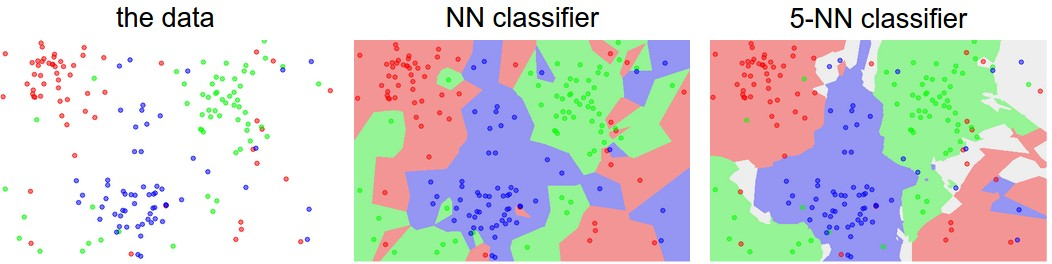
\includegraphics[width=1\textwidth]{knn}
	\caption{Porovnanie k-NN klasifikátorov\cite{odkaz:KnnImage}}
	\label{pic:kNN}
\end{figure}


\subsection{Support Vector Machines}
Support Vector Machines (SVM's) sú metódy učenia používané pre binárnu klasifikáciu.
Základnou myšlienkou je nájdenie hyper--roviny, ktorá perfektne oddelí \textit{d}--dimenzionálne dáta do dvoch tried\cite{prop:IntroductionToSVM}.
SVM sa snaží maximalizovať vzdialenosť medzi rozdeľujúcou rovinou a dátami nachádzajúcimi sa v každej z 2 polrovín\cite{prop:SupervisedMachineLearning}.
Avšak kedže vstupné dáta väčšinou nie su lineárne separovatelné, SVM's predstavujú pojem "jadrový priestor indukovaný príznakom"[eng. “kernel induced feature space”],
    ktorý prevádza dáta do vyššieho dimenzionálneho priestoru, kde dáta sú oddeliteľné.\cite{prop:IntroductionToSVM}

Ak trénovacie dáta sú lineárne separovatelné, tak dvojica $(w, b)$ existuje ako\cite{prop:SupervisedMachineLearning}:
\begin{equation}
    \label{eq:SVMPair1}
    w^T * x_i + b \geq 1, \; pre \; x_i \in P
\end{equation}
\begin{equation}
    \label{eq:SVMPair2}
    w^T * x_i + b \leq -1, \; pre \; x_i \in N
\end{equation}
s rozhodovacím pravidlom
\begin{equation}
    \label{eq:SVMDecisionRule}
    f_{w,b}(x) = sgn(w^T x + b)
\end{equation}
kde $w$ je váhový vektor a $b$ je predpoveď[eng. \#TODO biases asi] (alebo $-b$ je prahová hodnota).
V tomto prípade keď je možné lineárne rozdeliť dve triedy, tak optimálna hyper--rovina pre rozdelenie
    môže byť nájdena, minimalizáciou kvadratickej formy rozdeľujúcej hyper--roviny
\begin{equation}
    \label{eq:SVMDecisionRule}
    mininimize_{w,h} \; \Phi(w) = \frac{1}{2}||w||^2, \; pre \; y_i(w^Tx_i + b) \geq 1, i = 1, \dots, l
\end{equation}

V tomto prípade lineárneho rozdelenia dát, pri nájdení optimálnej rozdeľujúcej hyper--roviny, dátove body, ktoré ležia na jej okraji
    sa nazývajú podporné vektorové body[eng. support vector points] a riešenie je reprezentované ako lineárna kombinácia iba 3 týchto bodov(vid. obrázok \ref{pic:SVMMAxMargin} ).
Ostatné body sú ignorované\cite{prop:SupervisedMachineLearning}.

\begin{figure}[H]
	\centering
	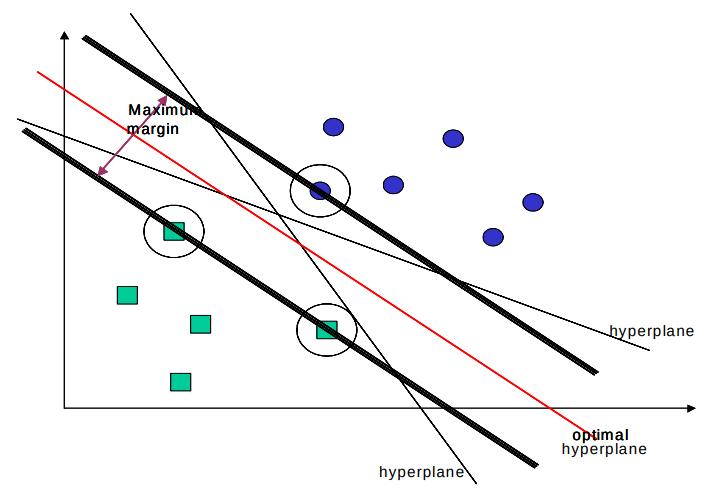
\includegraphics[width=1\textwidth]{SVM_max_margin}
	\caption{Maximálne rozpätie\cite{prop:SupervisedMachineLearning}}
	\label{pic:SVMMAxMargin}
\end{figure}

Avšak väčsina reálnych problémou zahŕňa nelineárne rozdelenie dát pre ktoré neexistuje žiadna hyper--rovina, ktorá by úspešne rozdelila trénovacie dáta.
Riešenie tohto problému je mapovať dáta do vyššie--dimenzionálneho priestoru a definovať tam rozdeľujúcu hyper--rovinu.
Tento vyššíe-dimenzionálny priestor je nazývaný transformovaný priestor príznakov[eng. transformed feature space], ako opak ku vstupnému priestoru[eng. input space] obsahujúcemu trénovacie dáta\cite{prop:SupervisedMachineLearning}.

Pri vhodne zvolenom transformovanom priestore príznakov dostatočnej veľkosti, môžu byť všetky trénovacie dáta rozdelitelné.
Lineárne rozdelenie v transformovanom priestore príznakov zodpovedá nelineárnemu rozdeleniu v pôvodnom vstupnom priestore.

Mapovanie dát do určitého Hilbertovho priestora \cite{prop:HilbertSpace} $H$ ako $\Phi:R^d \rightarrow H$.
Potom trénovací algoritmus závisý len na údajoch zo skalárneho súčinu[eng. dot products] v priestore $H$, t.j na funkciách v tvare $\Phi(x_i) * \Phi(x_j)$.
Ak bude existovať "funkcia jadra"[eng. kernel function] $K$ ako $K(x_i, x_j) = \Phi(x_i)*\Phi(x_j)$, tak budeme musieť použiť iba funkciu $K$ v trénovacom algoritme
    a nikdy nebudeme potrebovať explicitne definovať $\Phi$\cite{prop:SupervisedMachineLearning}.

Takže jadrá[eng. kernels] sú špeciálnou triedou funkcií, ktoré dovoľujú, aby sa vnútorné produkty vypočítali priamo vo funkčnom priestore[eng. feature space] bez toho, aby sa vykonalo vyššie popísané mapovanie.
Po vytvorení hyper--roviny sa funkcia jadra použije na mapovanie nových bodov do funkčného priestoru pre klasifikáciu\cite{prop:SupervisedMachineLearning}.

Voľba správnej funkcie jadra je veľmi dôležitá, kedže definujú transformovaný priestor príznakov v ktorom budú trénovacie dáta klasifikované.
Genton \cite{prop:KernelClasses} popísal niekoľko tried jadier, avšak, neadresoval otázku, ktorá trieda je najvhodnejšie pre daný problém.

Zoznam populárnych jadier\cite{prop:SupervisedMachineLearning}:
\begin{equation}
    K(x, y) = (x*y+1)^P
\end{equation}
\begin{equation}
    K(x, y) = e^{\frac{-||x-y||^2}{2 \sigma^2}}
\end{equation}
\begin{equation}
    K(x, y) = tanh(\kappa x*y - \delta)^P
\end{equation}

\begin{figure}[H]
	\centering
	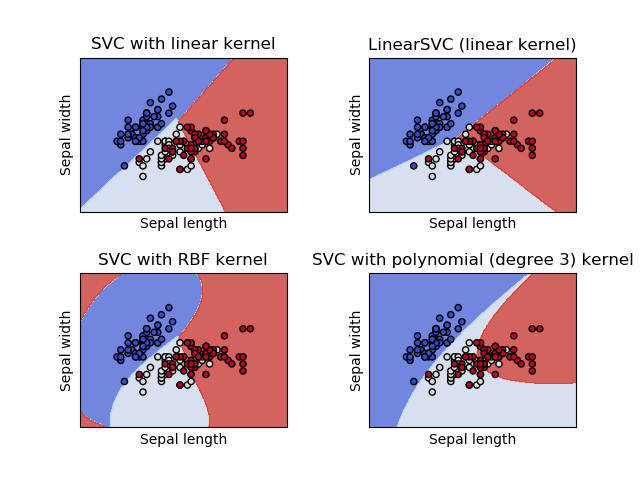
\includegraphics[width=1\textwidth]{sphx_glr_plot_iris_0012}
	\caption{Porovnanie rôznych typov SVM klasifikátorov\cite{odkaz:SVMImage}}
	\label{pic:SVMComparison}
\end{figure}


\subsection{Stochastic Gradient Descent}
Výpočtova zložitosť algoritmou učenia sa stáva kritickým obmedzujúcim faktorom, pri používaní veľmi rozsiahlých množín dát.
Preto pre veľké množíný dát sa začal používať Stochastic Gradient Descent\cite{prop:StochasticGradientDescent}, ktorý tieto výpočty dokáže optimalizovať.

Každý vzor $z$ je pár $(x, y)$ kde $x$ je ľubovolný vstup a $y$ skalárny výstup.
Máme stratovú funkciu [eng. loss function] $\ell(\hat{y},y)$ ktorá meria hodnotu predpovedania $\hat{y}$ keď správna odpoveď je $y$,
    a zvolíme si rodinu $\mathcal{F}$ funkcií $f_w(x)$ parametrizované váhovym vektorom $w$.

Hľadáme funkciue $f \in \mathcal{F}$, ktorá minimalizuje stratu $Q(z,w) = \ell(f_w(x), y)$ spriemerovanú vzhlaďom na vzory $z$.
Avšak pre napodobenie príprody je prirodzenejšie priemerovať vzhľadom na neznámu distribúciu $dP(z)$\cite{prop:StochasticGradientDescent}.
\begin{equation}
    E(f) = \int{\ell(f(x), y)dP(z)} \quad E_n(f) = \frac{1}{n}\sum_{i=1}^{n}\ell(f(x_i), y_i)
\end{equation}
$E_n(f)$ meria výkonnosť trénovacích dát. $E(f)$ meria generalizovanú výkonnosť, teda očakávaný výkon v budúcich vzorkách.

Pomocou klesania gradientu[eng. gradient descent] minimalizujeme $E_n(f_w)$, kde každá iterácia aktualizuje váhove vektory $w$ na základne gradientu.
\begin{equation}
    w_{t+1} = w_t - \gamma \frac{1}{n}\sum_{i=1}^{n}\bigtriangledown_w Q(z_i, w_t)
\end{equation}
kde $\gamma$ je vhodne zvolený zisk[eng. gain].

Stochastic Gradient Descent algoritmus je drastické zjednodušenie.
Namiesto počítania gradientu pre $E_n(f_n)$, každá iterácia odhadne tento gradient na základe jednej náhodne vybranej vzorky $z_t$\cite{prop:StochasticGradientDescent}:
\begin{equation}
    w_{t+1} = w_t - \gamma \bigtriangledown_w Q(z_t, w_t)
\end{equation}


\subsection{Neurónové siete}
Neurónová sieť (NN) je masívne paralelný procesor, ktorý má sklon k uchovávaniu experimentálnych znalostí a ich ďalšieho využívania.
Napodobňuje ľudský mozog v dvoch aspektoch \cite{odkaz:NNIntroduction}:
\begin{enumerate}
	\item[$\bullet$] poznatky sú zbierané v NN počas učenia
	\item[$\bullet$] medzineurónové spojenia (synaptické váhy - SV) sú využívané na ukladanie znalostí
\end{enumerate}
Toto je jedna z definícii NN, akceptovaná NN komunitou.
Je zrejmé, že inšpirácia ku vzniku NN prišla z biologických systémov.
Na prvý dojem vysoko abstraktná disciplína nachádza množstvo aplikácii v praxi a stáva sa prostriedkom pre riešenie problémou v širokom spektre odborných oblastí\cite{odkaz:NNIntroduction}.

Rôzne architektúry umelých neurónových sieti[eng. artificial neural network] sa používajú pre riešenie rôznych úloh.
Konvolučné a rekurentné NN sú dve z najúspešnejších a sú z veľkej časti zodpovedné za nedávnu revolúciu umelej inteligencie\cite{odkaz:CorrectionOfImageOrentation}.

Vo všeobecnosti môžeme vymenovať nasledovné oblasti využitia neurónových sieti\cite{odkaz:NNIntroduction}:
\begin{enumerate}
    \item[$\bullet$] klasifikácie do tried, klasifikácia situácií
    \item[$\bullet$] riešenie predikčných problémou
    \item[$\bullet$] problémy riadenia procesov
    \item[$\bullet$] tranformácia signálov
\end{enumerate}

Neurónové siete sú usporiadané do vnútorne prepojených vrstiev umelých neurónov.
Jednoducho povedané, každá vrstva berie výstup z prechádzajucej vrstvy, aplikuje transformácie a výsledok pošle na vstup ďalšej vrstve.
Prvá vrstva vstupov je prepojená na vstupné dáta, ktoré sa majú spracovať a posledná vrstva je akýkoľvek výstup, ktorý chceme predpovedať \cite{odkaz:CorrectionOfImageOrentation} (vid. obrázok \ref{pic:NNExample}).
\begin{figure}[H]
	\centering
	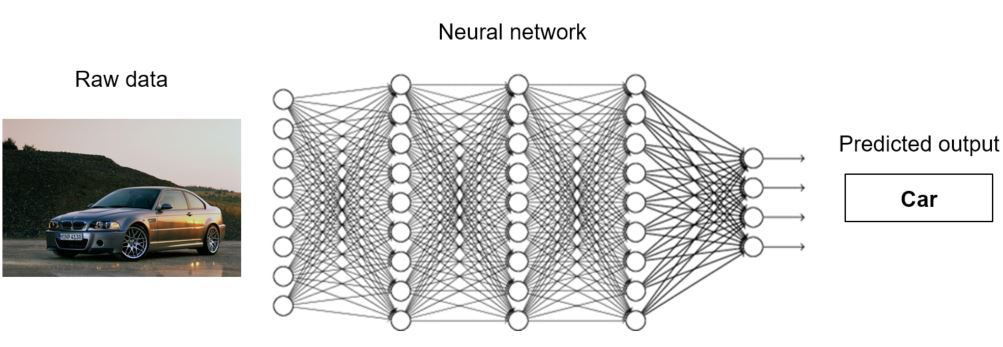
\includegraphics[width=1\textwidth]{nn}
	\caption{Jednoduchá architektúra NN s 1 vstupnou, 3 skrytímy a 1 výstupou vrstvou\cite{odkaz:CorrectionOfImageOrentation}}
	\label{pic:NNExample}
\end{figure}

\subsubsection{Perceptron}
Pre pochopenie fungovania neurónovej siete je potrebné najprv pochopiť umelý neurón, zvaný perceptron.
Perceptron vynašiel vedec Frank Rosenblatt v 1950 až 1960 roku, inšpirovaný predchádzajucov prácov Warren McCulloch a Walter Pitts.
Dnes sa bežné používa iný model umelého neurónu tzv. sigmoid neurón\cite{odkaz:HandwrittenDigitRecognision}.

V jednoduchosti, perceptron zoberie niekoľko vstupov, $x_1, x_2, \dots$ a reprodukuje ich na jediný binárny výstup.
\begin{figure}[H]
	\centering
	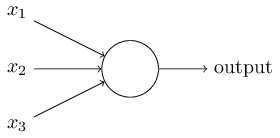
\includegraphics[width=0.4\textwidth]{tikz0}
	\caption{Jednoduchý príklad perceptronu\cite{odkaz:HandwrittenDigitRecognision}}
	\label{pic:Perceptron}
\end{figure}
Rosenblatt navrhol jednoduché pravidlo pre výpočet výstupu.
Zaviedol váhy[eng. weights], $w_1, w_2, \dots$,
Reálne čisla ktoré vyjadrujú dôležitosť príslušných vstupov vzhľadom na výstupy.
Výstup neurónu, 0 alebo 1, sa určuje podľa toho či vážena suma $\sum_j w_j x_j$ je menšia alebo väčsia ako určitá prahová hodnota.
Matematické vyjadrenie aktivačnej funkcie perceptronu by potom bolo\cite{odkaz:HandwrittenDigitRecognision}:
\begin{equation}
    output = 0, \; ak \; \sum_j w_j x_j \leq threshold
\end{equation}
\begin{equation}
    output = 1, \; ak \; \sum_j w_j x_j > threshold
\end{equation}

Matematický model perceptronu je možné zjednodušiť a to prepísaním formuly $\sum_j w_j x_j$ na skalárny súčin[eng. dot product],
    $w*x \equiv \sum_j w_j x_j$, kde $w$ a $x$ sú vektory váh a vstupov.
Druhá zmena je presun prahovej hodnoty na opačnú stranu nerovnice, a nahradiť ju tzv. perceptron bias, $b \equiv -threshold$.
Použitím týchto úprav bude model vyzerať nasledovne\cite{odkaz:HandwrittenDigitRecognision}:
\begin{equation}
    output = 0, \; ak \; w*x + b \leq 0
\end{equation}
\begin{equation}
    output = 1, \; ak \; w*x + b > 0
\end{equation}

\begin{figure}[H]
    \centering
    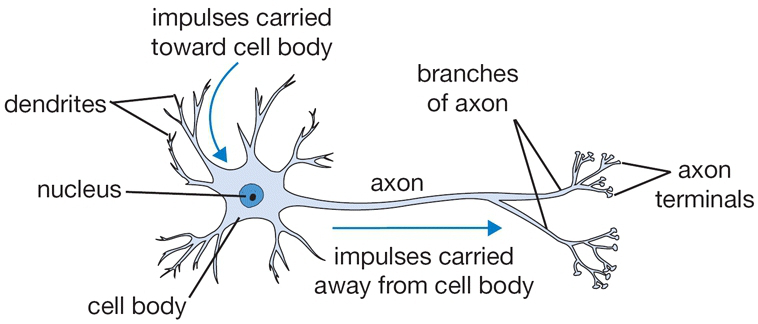
\includegraphics[width=0.5\textwidth]{neuron}
    \qquad
    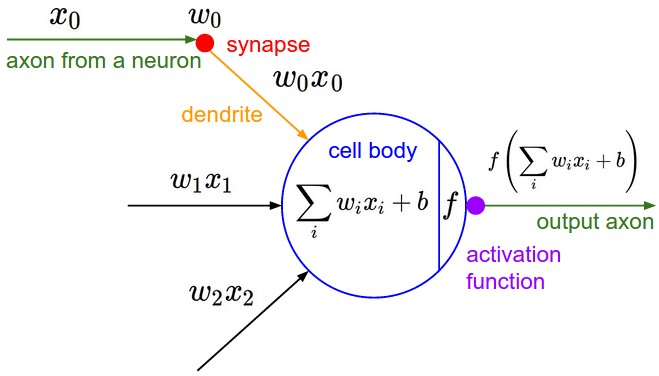
\includegraphics[width=0.4\textwidth]{neuron_model}
    \caption{biologický neurón(vľavo) a jeho matematický model(vpravo)\cite{odkaz:ConvolutionalNeuralNetworkCS231n}}
    \label{pic:Neuron}
\end{figure}

\subsubsection{Sigmoid}
Sigmoid je jedna z aktivačných funkcií používana v neúronových sietach, jej matematická formula je
\begin{equation}
    \sigma(x) = \frac{1}{1 + e^{-x}}
\end{equation}
je zobrazená na obrázku \ref{pic:ActivationFunctions} vľavo.

Funkcia zoberie skutočné číslo a "stlačí"[eng. squashes] ho do rozmedzia 0 až 1.
Kde veľké záporne čísla nadobudnú hodnotu 0 a veľke kladné pozitívne čísla hodnotu 1.
Funkcia sigmoid sa historicky často používala pretože má peknú interpretáciu pre spúštanie "výstrelu" neurónu,
    od nevýpalanie (0) až po úplne nasýtenie strely pri predpokladanej maximálnej frekvancií (1).
V praxi, sa sigmoid používa už len zriedka.
Pretože ma 2 hlavné nevýhody\cite{odkaz:ConvolutionalNeuralNetworkCS231n}:
\begin{enumerate}
    \item[$\bullet$] \textbf{Zabíjanie gradientov} - keď sa aktivácia neurónu nasýti na obidvoch koncoch 0 alebo 1, gradient v týchto oblastiach je takmer nulový.
    Tento gradient sa používa pri spätnej propagácií[eng. backpropagation] v neurónových sietach. Preto ak je miestny gradient veľmi malý, takmer žiaden signál
    neurónom nepreteká k jeho váham a rekurzívne k jeho dátam. Taktiež ak pri inicializácií sú váhy príliš veľké, väčsina neurónov by bolo nasýtených a sieť by sa sotva niečo učila.
    \item[$\bullet$] \textbf{Výstupy nie sú centrované na nulu} - to má dôsledky na dynamiku pri klesaní gradient-u, pretože ak sú údaje prichádzajúce do neurónu vždy kladné,
    potom gradient na váhach $w$ nadobudne, počas spätnej propagáciie, všetky hodnoty pozitívne alebo negatívne (v závisloti na gradient-e celého výrazu $f$).
    To by mohlo viesť k nežiadúcej cik-cakovitej dynamike pri aktualizáciach gradient-ov pre váhy.
\end{enumerate}


\subsubsection{Tanh}
Funkcia tanh dalšia z aktivačných funkcií neurónu je zobrazená na obrázku \ref{pic:ActivationFunctions} vpravo.
Tanh zoberie skutočné čislo a stlačí ho do rozmedzia -1 až 1. Pracuje podobne ako sigmoid.
Matematický zápis je\cite{odkaz:ConvolutionalNeuralNetworkCS231n}:
\begin{equation}
    tanh(x) = 2\sigma(2x) - 1
\end{equation}
Kedže netrpí nevýhodami ako sigmoid tak v praxi je preferovanejší.


\begin{figure}[H]
    \centering
    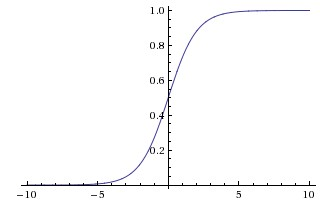
\includegraphics[width=0.45\textwidth]{sigmoid}
    \qquad
    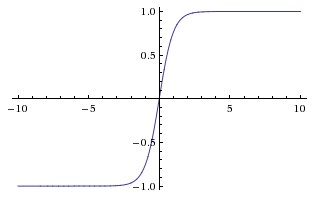
\includegraphics[width=0.45\textwidth]{tanh}
    \caption{
        Vľavo: Sigmoid nelineárne stlačenie čísel do rozsahu [0,1],
        Vpravo: Tanh nelineárne stlačenie čísel do rozsahu [-1,1] \cite{odkaz:ConvolutionalNeuralNetworkCS231n}
    }
    \label{pic:ActivationFunctions}
\end{figure}

\subsubsection{ReLU a Leaky ReLU}
V praxi existuje niekoľko dalšich aktivačných funkcií, každá je použitelná pre riešenie iného problému,
    čiže každá ma svoje výhody ale aj nevýhody.
Ako príklad môžeme uviesť ReLU (Rectified Linear Unit)
\begin{equation}
    f(x) = max(0,x)
\end{equation}
alebo jeho obdobu Leaky ReLU, ktorá sa snaží vyriešiť nevýhody ReLU.
\begin{equation}
    f(x) = x \quad ak \; x > 0
\end{equation}
\begin{equation}
    f(x) = ax \quad ak \; x <= 0
\end{equation}
kde $a$ je malá konštanta (napr. 0.01) \cite{odkaz:ConvolutionalNeuralNetworkCS231n}.

\subsubsection{Architektúra neurónovej siete}
Ako bolo spomínane už vyššie, neúronova sieť je modelovaná ako kolekcia neurónov, ktoré sú prepojené v acyklickom grafe.
Modely neúronovych sieti sú často organizované do odlišných vrstiev neurónov.
Pre bežné neúronove siete je najbežnejšou vrstvou tzv. plne-prepojená vrstva [eng. fully-connected layer],
    v ktorej sú neuróny medzi dvoma priľahlými vrstvami plne párovo prepojené, ale neuróny v jeden vrstve nemajú medzi sebou žiadne spojenia.
Na obrázku \ref{pic:NeuralNetworkArchitecture} nižšie sú uvedené dve topológie ktoré využívajú plne-prepojené vrstvy\cite{odkaz:ConvolutionalNeuralNetworkCS231n}:
\begin{figure}[H]
    \centering
    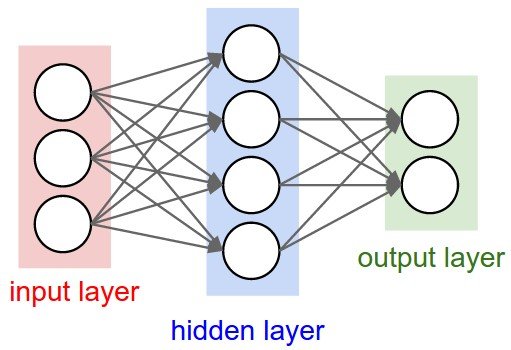
\includegraphics[width=0.38\textwidth]{neural_net}
    \qquad
    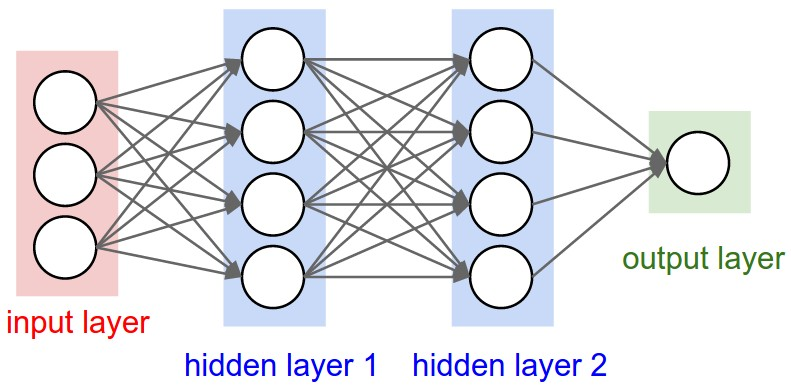
\includegraphics[width=0.52\textwidth]{neural_net2}
    \caption{Vľavo: 2-vrstvová neurónová sieť, Vpravo: 3-vrstvová neurónová sieť \cite{odkaz:ConvolutionalNeuralNetworkCS231n}}
    \label{pic:NeuralNetworkArchitecture}
\end{figure}

Vačšie neúronove sieťe dokážu reprezentovať komplikovanejšie funkcie.
Na obrázku \ref{pic:XNNLayerExample} je vidieť rozdiel klasifikácie dát do 2 tried (červená, zelená) použít rôznych veľkostí neúronových sieti.
\begin{figure}[H]
	\centering
	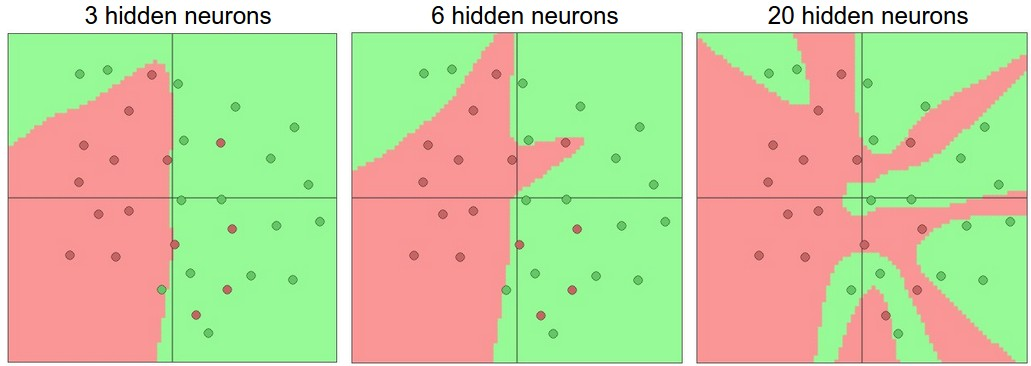
\includegraphics[width=1\textwidth]{layer_sizes}
	\caption{Zobrazenie klasifikácie dát rôznymi veľkostami NN \cite{odkaz:ConvolutionalNeuralNetworkCS231n}}
	\label{pic:XNNLayerExample}
\end{figure}

\subsection{Konvolučné neurónové siete}
Konvolučné neurónové siete [eng. convolutional neural networks] (CNNs), sú špeciálnym prípadom neurónových sieti pre spracovanie
    dát ktoré mau známu topológie podobnú mriežke.
Pre príklad je možné uviesť napríklad 2-dimenzionálne dát ako sieť pixelov pri spracovaní obrázkov.
Názov týchto sieti \textit{konvolučné} indikuje že používajú matematickú operáciu zvanú konvolúcia[eng. convolution]\cite{book:Goodfellow-et-al-2016}.

\subsubsection{Konvolúcia}
Vo svojej najobecnejšej podobe, konvolúcia je operácie dvoch funkcií s reálnymi hodnotami argumentov.
Operácia konvolúcie je typicky označovaná hviezdičkov:
\begin{equation}
    s(t) = (x * w)(t)
\end{equation}
V terminilógií konvolucnej siete je prvý argument (v tomto príklade funkcie $x$) sa často označuje ako vstup a druhý
    argument (v tomto príklade funkcia $w$) ako jadro[eng. kernel]. Výstup je niekedy označovaný ako mapa príznakov.

Bežne konvolúciu používa na viac ako jedej osy súčasne.
Pri použítí 2-dimenzionálne obrázku $I$ ako náš vstup, tak budeme chcieť použiť aj 2-dimenzionálne jadro $K$\cite{book:Goodfellow-et-al-2016}:
\begin{equation}
    S(i,j) = (I * K)(i, j) = \sum_m \sum_n I(m,n) K(i - m, j - n)
\end{equation}

Avšak množstvo knižníc ktoré implmentujú neúronove siete, používaju tzv. cross-correlation funkciu\cite{book:Goodfellow-et-al-2016}:
\begin{equation}
    S(i,j) = (I * K)(i, j) = \sum_m \sum_n I(i + m, i + n) K(m, n)
\end{equation}

\subsubsection{Architektúra}
CNN využívajú skutočnosti, že vstup pozostáva z obrázkov.
Na rozdiel od obyčajnej neurónovej siete majú vrstvy CNN neuróny usporiadané v troch rozmeroch: šírka, výška, hĺbka[eng. width, height, depth].
Hĺbka odkazuje na 3.dimenziu aktivačného zväzku[eng. activation volume], nie ne celkovú hĺbku neurónovej siete.
Neuróny vo vrtsve budú prepojené iba k malej oblasti vrstvy pred ňou, namiesto plného prepojenia \cite{odkaz:CNNArchitecture}.

Pre stavbu CNN sa využívajú 3 základne typy vrstiev:
\begin{enumerate}
    \item[$\bullet$] \textbf{Convolutional layer} - konvolučná vrstva je hlavný stavebný blok CNN, ktorá robí väčšinu výpočtov.
    Parametre tejto vrstvy pozostávajú zo súboru filtrov ktoré sa dokážu učit.
    Takto naučené filtre sa aktivujú keď uvidia určitý typ vizuálneho prvku, napr. hranu určitej orientácie alebo škvrnu určitej farby a pod..
    \item[$\bullet$] \textbf{Pooling layer} - túto vrstvu je obvyklé vkladať ako spojenie medzi dvoma konvolučnímy vrstvami.
    Jej funkciou je postupné znižovanie priestorovej veľkosti reprezentovaného vstupu, pre zníženie množstva parametrov a výpočtov v sieti, a teda aj kontroly pretrénovania.
    \item[$\bullet$] \textbf{Fully-Connected layer} - rovnako ako v obvyklých neúronových sietach, je to vrstva kde všetky neuróny sú prepojené s predchádzajucou vrstvou.
\end{enumerate}

\begin{figure}[H]
	\centering
	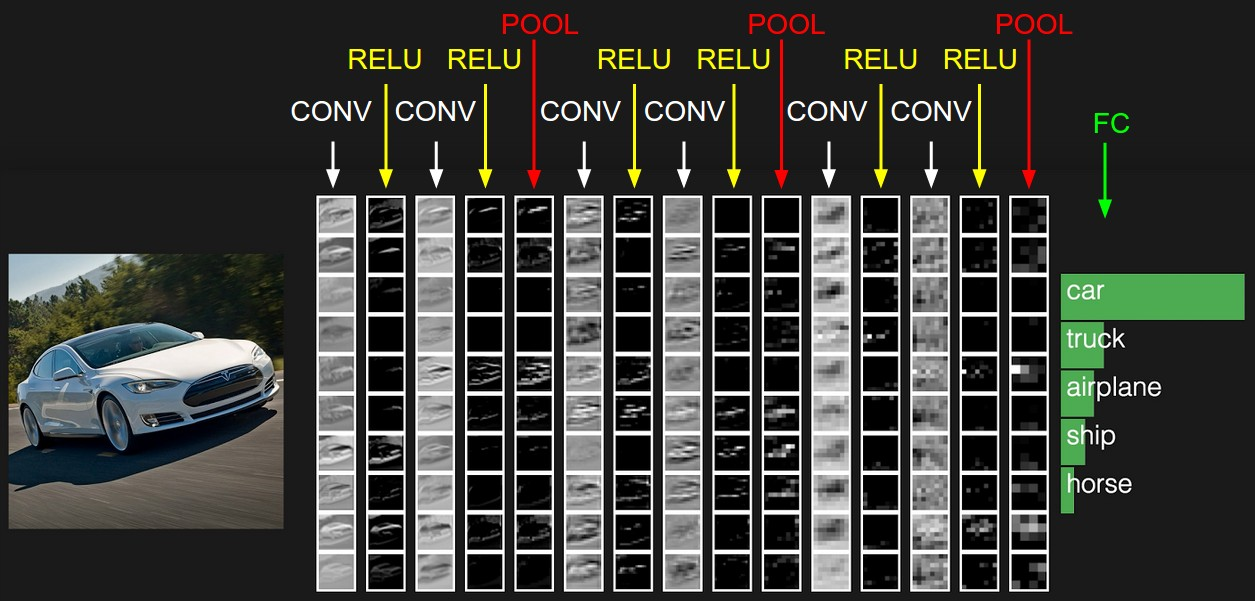
\includegraphics[width=1\textwidth]{convnet}
	\caption{Príklad architektúry konvolučnej neúronovej siete \cite{odkaz:CNNArchitecture}}
	\label{pic:CNNExample}
\end{figure}

\section{Predspracovanie obrazu}
%http://scikit-image.org/docs/dev/auto\_examples/
% Normalizacia obrazu - github ten kurz c231n - 17150\_FULLTEXT.pdf (normalization)
%\subsection{Hogova transformacia}
% - F3-DP-2016-Erlebach-Jonas-Automaticka detekce pupily v obraze.pdf
%\subsection{Detekcia hran}
%- Sobelov filter - podľa knižky patri medzi najpopulárnejšie hranové filter. Urobiť z neho magnitúdu obrazu potom.

\subsubsection{Rovnomerný pomer strán}
Pre sprcovanie obrazkou pomocou neúronových sieti je potrebné zabezpečiť aby každý obrázok mal rovnakú veľkosť a rovnaký pomer strán.
Väčšina modelov neurónovej siete predpokladá štvorcový vstupný obraz \cite{odkaz:NNPreprocessing}.

\subsubsection{Priemerna štandartná odchylka vstupných údajov}
Je užitočné vytvoriť si tzv. "stredný obraz" získaný priemernými hodnotami pre každý pixel zo všetkých trénovacích dát.
Tímto spôsobom je možné vytvoriť si základny prehľad o štruktúre vstupných dát.
Na základe toho môžeme potom do vstupným dát pridať rôzne dalšie variácie klasifikovaných objektov pre lepšie generalizovanie klasifikátora \cite{odkaz:NNPreprocessing}.

\subsubsection{Šedotónový obraz}
Dalším možnou technikou je vytvorenie šedotónového obrazu, kde všetky 3 zložky farby (RGB) zlúčime do jednej, šedotónovéj.
\begin{figure}[H]
	\centering
	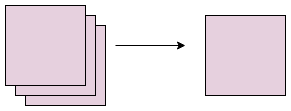
\includegraphics[width=0.4\textwidth]{grayscale}
	\caption{Prevod do šedotónového obrazu[eng. grayscaling]\cite{odkaz:NNPreprocessing}}
	\label{pic:GrayScaling}
\end{figure}

\subsubsection{Rožírenie vstupných dát}
Ďalšou bežnou technickou predspracovanie dát je rožšírenie existujúceho súboru dát s rôznymi variáciami existujúcich obrázkov.
Tieto variácie môžu zahŕňať zväčšovanie, zmenšovanie, rotačné zmeny a iné transformácie obrázkou.
Tento postup znižuje šancu že neúronová sieť rozpozná nežiadúce charakteristiky v množine vstupných dát \cite{odkaz:NNPreprocessing}.

% ------------ NEW CHAPTER ------------
\chapter{Návrh riešenia}

V tejto kapitole si priblížime navrhované technológie pre riešienie problému, tejto práce.
Kapitola zahŕňa popis knižníc pre strojové učenie ako je Tensorflow a Keras ktorý zovšeobecnuje a používa Tensorflow pre svoju prácu.
Následne nástroj scikit-learn ktorý budeme používať pre jednoduchú klasifikáciu pomocou postup ktoré boli vysvetlené v kapitole \ref{chap:technologie}.

\section{Tensorflow a Keras}

\subsubsection{Tensorflow}
TensorFlow je softvérová knižnica s otvoreným zdrojovým kódom[eng. open source library] pre numerické výpočty pomocou dátových vývojovím diagramov[eng. data flow graphs].
Uzly v grafe reprezentujú matematické operácie, zatiaľ čo hrany grafu reprezentujú multidimenzionálne dátové polia (tensors), ktoré medzi sebou kominukujú.
Flexibilná architektúra umožnuje nasadenie na viacerých CPU alebo GPU, serveroch alebo aj mobilných zariadeniach.
TensorFlow bol pôvodne vyvinutý na účely výskumu strojového učenia a výskumu hlbokých neurónových sieti, systém je dostatočne všeobecný aby bol aplikovaný v mnohých iných oblastiach \cite{odkaz:TensorFlow}.

\subsubsection{Keras}
Vysoká všeobecnosť knižice TensorFlow pre jej širokú aplikáciu, robí jej použitie pre tvornu neurónových sieti komplikovanejšiu.
Kde Keras bol postavený nad TensorFlow ktorý využíva ako svoj backend a tvorbu neurónových sieti zjednodušil.
Za jeho backend je možné použiť aj CNTK alebo Theona.
Táto implementácia knižnice Keras robí experimentovanie s NN jednoduchšiu a rýchlejšiu.
Aj keď sa snaží implementáciu zjednodušiť tak stále si zachováva modularitu a preto je možné dostatočne dobre modely NN upravovať a prisposobovať pre riešienie rôznych problémou \cite{odkaz:Keras}.

\section{scikit-learn}
Scikit-learn je softvérová knižica pre strojové učenie pre programovací jazyk Python.
Obsahuje množstvo algoritmou pre klasifikáciu, regresiu alebo zhlukovanie dát \cite{odkaz:scikitlearn}.
Pre riešenie tejto práce obsahuje vhodné triedy ktoré implementujú spomínane postupy zo sekcie \ref{sec:klasifikacia}.
Príklady tried pre jednotlivé algoritmy:
\begin{enumerate}
    \item[$\bullet$] \textbf{Nearest Neighbors} - scikit-learn poskytuje 2 rôzne klasifikátory pre algoritmus najbližsieho suseda.
    Trieda \textit{KNeighborsClassifier} klasifikuje na základe $k$ najbližšich susedov, kde $k$ je celé číslo špecifikované užívateľom.
    Druhá trieda \textit{RadiusNeighborsClassifier} implementuje klasifikáciu na základe počtu susedov v rámci pevného polomeru $r$ každého trénovacieho bodu,
    kde $r$ je hodnota s pohyblivou desatinou čiarkou určená užívateľom\footnote{\url{http://scikit-learn.org/stable/modules/neighbors.html\#nearest-neighbors-classification}}.
    \item[$\bullet$] \textbf{Support Vector Machines} - \textit{SVC}, \textit{NuSVC} a \textit{LinearSVC} sú triedy pre viac-triednu klasifikáciu.
    Pre ktoré je možné použit rôzne typy jadier[eng. kernels] \footnote{\url{http://scikit-learn.org/stable/modules/svm.html\#custom-kernels}}.
    \item[$\bullet$] \textbf{Stochastic Gradient Descent} - \textit{SGDClassifier} podporuje viac-triednu klasifikáciu pomocou kombinácie viacerých binárnych klasifikátorov v tzv.“one versus all” (OVA) schéme \footnote{\url{http://scikit-learn.org/stable/modules/sgd.html\#stochastic-gradient-descent}}.
\end{enumerate}

\section{Klasifikácia typu zbrane}
%- Exploiting-the-complementary-strengths-of-multi-layer-CNN-image-retrieval.pdf, preco pouzivat CNN na tento problem
%- Pouzit vsetky veci z teorie, pri SGD pre vacsi dataset.

\section{Určenie natočenia zbrane}


% ------------ NEW CHAPTER ------------
\pagebreak
\chapter{Implementácia}

\section{Databáza zbraní}
- ....
